\section{Rauschen in analogen Systemen}Siehe Kapitel \ref{ZF_rauschen} für einige nützlichen vereinfachten Formeln
\subsection{Rauschen}
Bei \textbf{weissem Rauschen} ist der Leistungsdichtespektrum im Spektrum konstant. $R_{xx}(\tau) = \frac{\eta}{2}\delta(\tau)$

\begin{center}
	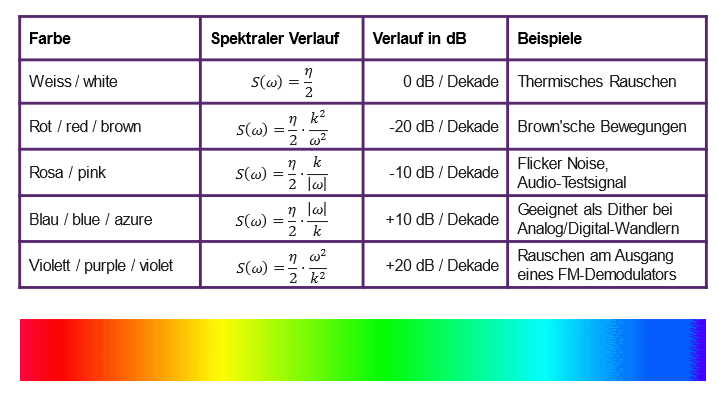
\includegraphics[width=\columnwidth]{Images/rauschen}
\end{center}

\subsection{SNRo}
Signal-to-Noise-Ratio ist ein Mass für die Übertragungsqualität:
\[
SNR_o = \left(\frac{S}{N}\right)_o = \frac{E[X_0^2(t)]}{E[N_o^2(t)]}
\]

Für konkrete SNRo siehe \script{174}ff